\documentclass{mimosis}

\usepackage{metalogo}

%%%%%%%%%%%%%%%%%%%%%%%%%%%%%%%%%%%%%%%%%%%%%%%%%%%%%%%%%%%%%%%%%%%%%%%%
% Some of my favourite personal adjustments
%%%%%%%%%%%%%%%%%%%%%%%%%%%%%%%%%%%%%%%%%%%%%%%%%%%%%%%%%%%%%%%%%%%%%%%%
%
% These are the adjustments that I consider necessary for typesetting
% a nice thesis. However, they are *not* included in the template, as
% I do not want to force you to use them.

% This ensures that I am able to typeset bold font in table while still aligning the numbers
% correctly.
\usepackage{etoolbox}

\usepackage[binary-units=true]{siunitx}
\DeclareSIUnit\px{px}

\sisetup{%
  detect-all           = true,
  detect-family        = true,
  detect-mode          = true,
  detect-shape         = true,
  detect-weight        = true,
  detect-inline-weight = math,
}

%%%%%%%%%%%%%%%%%%%%%%%%%%%%%%%%%%%%%%%%%%%%%%%%%%%%%%%%%%%%%%%%%%%%%%%%
% Hyperlinks & bookmarks
%%%%%%%%%%%%%%%%%%%%%%%%%%%%%%%%%%%%%%%%%%%%%%%%%%%%%%%%%%%%%%%%%%%%%%%%

\usepackage[%
  colorlinks = true,
  citecolor  = RoyalBlue,
  linkcolor  = RoyalBlue,
  urlcolor   = RoyalBlue,
  ]{hyperref}

\usepackage{bookmark}

%%%%%%%%%%%%%%%%%%%%%%%%%%%%%%%%%%%%%%%%%%%%%%%%%%%%%%%%%%%%%%%%%%%%%%%%
% Bibliography
%%%%%%%%%%%%%%%%%%%%%%%%%%%%%%%%%%%%%%%%%%%%%%%%%%%%%%%%%%%%%%%%%%%%%%%%
%
% I like the bibliography to be extremely plain, showing only a numeric
% identifier and citing everything in simple brackets. The first names,
% if present, will be initialized. DOIs and URLs will be preserved.

\usepackage[%
  autocite     = plain,
  backend      = bibtex,
  doi          = true,
  url          = true,
  giveninits   = true,
  hyperref     = true,
  maxbibnames  = 99,
  maxcitenames = 99,
  sortcites    = true,
  style        = numeric,
  ]{biblatex}

%%%%%%%%%%%%%%%%%%%%%%%%%%%%%%%%%%%%%%%%%%%%%%%%%%%%%%%%%%%%%%%%%%%%%%%%
% Some adjustments to make the bibliography more clean
%%%%%%%%%%%%%%%%%%%%%%%%%%%%%%%%%%%%%%%%%%%%%%%%%%%%%%%%%%%%%%%%%%%%%%%%
%
% The subsequent commands do the following:
%  - Removing the month field from the bibliography
%  - Fixing the Oxford commma
%  - Suppress the "in" for journal articles
%  - Remove the parentheses of the year in an article
%  - Delimit volume and issue of an article by a colon ":" instead of
%    a dot ""
%  - Use commas to separate the location of publishers from their name
%  - Remove the abbreviation for technical reports
%  - Display the label of bibliographic entries without brackets in the
%    bibliography
%  - Ensure that DOIs are followed by a non-breakable space
%  - Use hair spaces between initials of authors
%  - Make the font size of citations smaller
%  - Fixing ordinal numbers (1st, 2nd, 3rd, and so) on by using
%    superscripts

% Remove the month field from the bibliography. It does not serve a good
% purpose, I guess. And often, it cannot be used because the journals
% have some crazy issue policies.
\AtEveryBibitem{\clearfield{month}}
\AtEveryCitekey{\clearfield{month}}

% Fixing the Oxford comma. Not sure whether this is the proper solution.
% More information is available under [1] and [2].
%
% [1] http://tex.stackexchange.com/questions/97712/biblatex-apa-style-is-missing-a-comma-in-the-references-why
% [2] http://tex.stackexchange.com/questions/44048/use-et-al-in-biblatex-custom-style
%
\AtBeginBibliography{%
  \renewcommand*{\finalnamedelim}{%
    \ifthenelse{\value{listcount} > 2}{%
      \addcomma
      \addspace
      \bibstring{and}%
    }{%
      \addspace
      \bibstring{and}%
    }
  }
}

% Suppress "in" for journal articles. This is unnecessary in my opinion
% because the journal title is typeset in italics anyway.
\renewbibmacro{in:}{%
  \ifentrytype{article}
  {%
  }%
  % else
  {%
    \printtext{\bibstring{in}\intitlepunct}%
  }%
}

% Remove the parentheses for the year in an article. This removes a lot
% of undesired parentheses in the bibliography, thereby improving the
% readability. Moreover, it makes the look of the bibliography more
% consistent.
\renewbibmacro*{issue+date}{%
  \setunit{\addcomma\space}
    \iffieldundef{issue}
      {\usebibmacro{date}}
      {\printfield{issue}%
       \setunit*{\addspace}%
       \usebibmacro{date}}%
  \newunit}

% Delimit the volume and the number of an article by a colon instead of
% by a dot, which I consider to be more readable.
\renewbibmacro*{volume+number+eid}{%
  \printfield{volume}%
  \setunit*{\addcolon}%
  \printfield{number}%
  \setunit{\addcomma\space}%
  \printfield{eid}%
}

% Do not use a colon for the publisher location. Instead, connect
% publisher, location, and date via commas.
\renewbibmacro*{publisher+location+date}{%
  \printlist{publisher}%
  \setunit*{\addcomma\space}%
  \printlist{location}%
  \setunit*{\addcomma\space}%
  \usebibmacro{date}%
  \newunit%
}

% Ditto for other entry types.
\renewbibmacro*{organization+location+date}{%
  \printlist{location}%
  \setunit*{\addcomma\space}%
  \printlist{organization}%
  \setunit*{\addcomma\space}%
  \usebibmacro{date}%
  \newunit%
}

% Do not abbreviate "technical report".
\DefineBibliographyStrings{english}{%
  techreport = {technical report},
}

% Display the label of a bibliographic entry in bare style, without any
% brackets. I like this more than the default.
%
% Note that this is *really* the proper and official way of doing this.
\DeclareFieldFormat{labelnumberwidth}{#1\adddot}

% Ensure that DOIs are followed by a non-breakable space.
\DeclareFieldFormat{doi}{%
  \mkbibacro{DOI}\addcolon\addnbspace
    \ifhyperref
      {\href{http://dx.doi.org/#1}{\nolinkurl{#1}}}
      %
      {\nolinkurl{#1}}
}

% Use proper hair spaces between initials as suggested by Bringhurst and
% others.
\renewcommand*\bibinitdelim {\addnbthinspace}
\renewcommand*\bibnamedelima{\addnbthinspace}
\renewcommand*\bibnamedelimb{\addnbthinspace}
\renewcommand*\bibnamedelimi{\addnbthinspace}

% Make the font size of citations smaller. Depending on your selected
% font, you might not need this.
\renewcommand*{\citesetup}{%
  \biburlsetup
  \small
}

\DeclareLanguageMapping{british}{bibliography-correct-ordinals}
\DeclareLanguageMapping{english}{bibliography-correct-ordinals}

\bibliography{Thesis}

%%%%%%%%%%%%%%%%%%%%%%%%%%%%%%%%%%%%%%%%%%%%%%%%%%%%%%%%%%%%%%%%%%%%%%%%
% Fonts
%%%%%%%%%%%%%%%%%%%%%%%%%%%%%%%%%%%%%%%%%%%%%%%%%%%%%%%%%%%%%%%%%%%%%%%%

\ifxetexorluatex
  % \setmainfont{Minion Pro}
  \setmainfont{Times New Roman}  

\else
  \usepackage[lf]{ebgaramond}
  \usepackage[oldstyle,scale=0.7]{sourcecodepro}
  \singlespacing
\fi

\renewcommand{\th}{\textsuperscript{\textup{th}}\xspace}

\newacronym[description={Principal component analysis}]{PCA}{PCA}{principal component analysis}
\newacronym                                            {SNF}{SNF}{Smith normal form}
\newacronym[description={Topological data analysis}]   {TDA}{TDA}{topological data analysis}

\newglossaryentry{LaTeX}{%
  name        = {\LaTeX},
  description = {A document preparation system},
  sort        = {LaTeX},
}

\newglossaryentry{Real numbers}{%
  name        = {$\real$},
  description = {The set of real numbers},
  sort        = {Real numbers},
}

\makeindex
\makeglossaries

%%%%%%%%%%%%%%%%%%%%%%%%%%%%%%%%%%%%%%%%%%%%%%%%%%%%%%%%%%%%%%%%%%%%%%%%
% Incipit
%%%%%%%%%%%%%%%%%%%%%%%%%%%%%%%%%%%%%%%%%%%%%%%%%%%%%%%%%%%%%%%%%%%%%%%%

\title{\texttt{latex-mimosis}}
\subtitle{A minimal, modern \LaTeX{} package for typesetting your thesis}
\author{Bastian Rieck}

\usepackage{listings}
\usepackage{xcolor}
\lstset{
    numbers=left, 
    numberstyle= \tiny, 
    keywordstyle= \color{ blue!70},
    commentstyle= \color{red!50!green!50!blue!50}, 
    frame=shadowbox, % 阴影效果
    rulesepcolor= \color{ red!20!green!20!blue!20} ,
    escapeinside=``, % 英文分号中可写入中文
    xleftmargin=2em,xrightmargin=2em, aboveskip=1em,
    framexleftmargin=2em
} 

\begin{document}

\frontmatter
  \begin{titlepage}
  \vspace*{5cm}
  \makeatletter
  \begin{center}
    \begin{Huge}
      \@title
    \end{Huge}\\[0.1cm]
    %
    \begin{Large}
      \@subtitle
    \end{Large}\\
    %
    \emph{by}\\
    \@author
    %
    \vfill
    A document submitted in partial fulfillment
    of the requirements for the degree of\\
    \emph{Technical Report}\\
    at\\
    \textsc{Miskatonic University}
  \end{center}
  \makeatother
\end{titlepage}

\newpage
\null
\thispagestyle{empty}
\newpage

  \begin{center}
  \textsc{Abstract}
\end{center}
%
\noindent
%
Scientific documents often use \LaTeX{} for typesetting. While numerous
packages and templates exist, it makes sense to create a new one. Just
because.


  \tableofcontents

\mainmatter

  \section{Preface}

This is a \LaTeX report written by Haodong Liao, a student of UESTC who participated the summer school of UCPH. More code of this summer school project can be seen at \href{https://github.com/Medill-East/ComputerScience/tree/master/Professional%20Core%20Courses/Functional%20Programming/SummerSchool}{MyRepository}.

\section{Introduction}

A list in F\# is an ordered, immutable series of elements of the same type\footnote[1]{https://docs.microsoft.com/en-us/dotnet/fsharp/language-reference/lists}, and some of the list funcions like map, fold and filter are very powerful for list processing. 

In this report, I replaced the library calls in \emph{myFold} and \emph{myFilter} with my own recursive implementations of these functions according to the assignment description, in detail, in both functions, I uesd \emph{match..with} to achieved pattern-matching and the idea of recrusion to implemented the functions.

All in all, results I achieved were as following:

\begin{itemize}
\item met the requirement of replacing the library calls in \emph{myFold} and \emph{myFilter} with my own recursive implementations of these functions,
\item used \emph{match..with} to achieved pattern-matching,
\item made program work by my own,
\item improved \emph{myFold} function to be more generic with the help of Prof.Sporring.
\end{itemize}

The remaining structure of the article is as follows. Section 3 states the problem in detail. Section 4 analysis and designs the problem. Section 5 describes the essential parts in my implementation. The program are evaluated in Section 6 and discussed in Section 7.

\section{Problem statement}

This assignment required us to replace the library function with recursive implementations for \emph{myFold} and \emph{myFilter} based on the file \emph{recursiveMapFoldFilter.fsx}, which is a fully functionning program must be compiled and executed from the console. 

This program takes 2 arguments: a string and a postive integer \emph{n}. The string can be either \emph{map}, \emph{fold}, or \emph{filter}. The output is a random list of length \emph{n} consisting of postive integers less than 10 and a processed list. For \emph{fold}, the random elements have been multiplied by 2 and their order have been reversed, and for \emph{filter}, only those elments larger than 4 have been included.

\section{Analysis and Design}

\subsection{Fold Function}

\lstset{language=Csh}
\begin{lstlisting}
List.fold: 
  f:('State -> 'T -> ' State) -> 
  elm:'State -> 
  lst: 'T list 
    -> ' State.
\end{lstlisting}

According to \cite{sporring2019}, List.fold function \emph{updates an accumulator iteratively by applying f to each element in lst}. 

So there were two branches needed to be handled, one is empty list, the other is list with element(s). For empty list, the return value couldn't be constrained to list and should be as same as accumulator. For list with element(s), fold function should be called recursively, the accumulator should always be the result of argument function which had parameters of accumulator and current element of list. The key part of the pseudocode is shown as following:

\begin{lstlisting}
Fold function accumulator list =
  match list with
    | emptylist -> return accumulator
    | list with element(s) -> 
        Fold function (result of function with current accumulator and element) restList
\end{lstlisting}

\subsection{Filter Function}

\lstset{language=Csh}
\begin{lstlisting}
List.filter: 
  f:('T -> bool) -> 
  lst:'T list 
    -> 'T list
\end{lstlisting}

According to \cite{sporring2019}, List.filter function \emph{returns a new list with all the elements of lst for which f evaluates to true}. 

Same as fold function, there were two branches needed to be handled. For empty list, the return value should be the empty list itself. For list with element(s), filter function should be called recursively according to the bool expression, if the value was true, not only should we call the filter function recursively, the current element should be a part of result list. If the value of bool expression is false, there was no need to care about current element.The key part of the pseudocode is shown as following:

\begin{lstlisting}
Filter boolexpression list =
  match list with
    | emptylist -> return emptylist
    | list with element(s) -> 
        if boolexpression is true
        then
          concat current element 
          and call Filter function with boolexpression and rest list
        else
          call Filter function with boolexpression and rest list  

\end{lstlisting}

\section{Program description}

\subsection{Fold function}

My implementation of fold function was as follows:

\begin{lstlisting}
let rec myFold (f: 'b -> 'a -> 'b) (acc: 'b) (lst: 'a list) : 'b =
  match lst with
    | [] -> acc
    // second time wrong
    // [] -> []
    | elm::rest -> 
        // first time wrong
        //let result = myFold f acc rest @ (f acc elm)
        //result
        let result = myFold f (f acc elm) rest
        result
\end{lstlisting}

As it shows, to my point of view, the place I made mistake was the key of this function, whether for empty list or list with element(s), a problem I met was constrained the type of return value. It was a subtle but vital problem.

\subsection{Filter function}

My implementation of filter function was as follows:


\lstset{language=Csh}
\begin{lstlisting}
let rec myFilter (p: 'a -> bool) (lst: 'a list) : 'a list =
  //List.filter p lst
  match lst with
  | [] -> []
  | elm::rest -> 
    if (p elm)
    then 
        [elm] @ (myFilter p rest)
    else 
        myFilter p rest
\end{lstlisting}

I was struggled in the code of list with element(s) when I started to solve this problem, but it was much easier when I figured out the reason confused me was that I was so obsessed with recursion and ignored the thinking of boolean expressions. Things went smoothly when I rearranged my thoughts.

\section{Evaluation}

The testing environment was macOS Mojave 10.14.5 system with iTerm and Microsoft (R) F\# Compiler version 4.1.

\subsection{Fold function}

I complied and tested the fold function with parameter \emph{fold 9}, and the result was correct:

\begin{figure}[h]
      \centering
      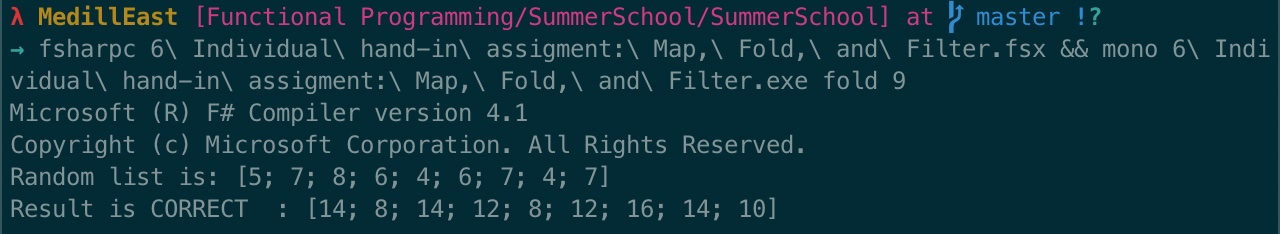
\includegraphics[width=\linewidth]{fold}
      \caption{Testing of fold function}
      \label{fig:fold}
\end{figure}

\subsection{Filter function}

I complied and tested the filter function with parameter \emph{filter 9}, and the result was correct:

\begin{figure}[h]
      \centering
      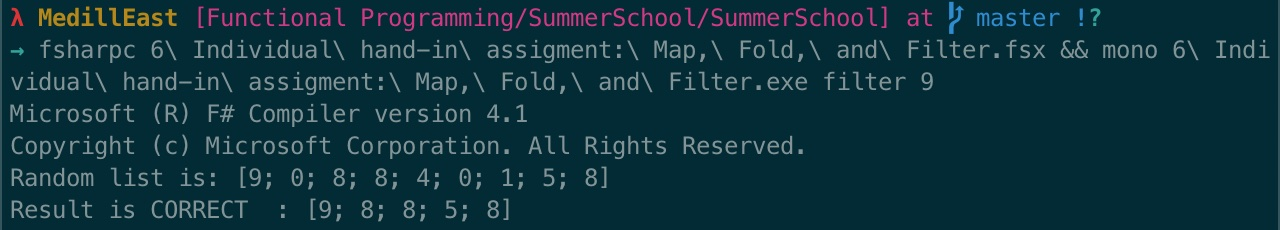
\includegraphics[width=\linewidth]{filter}
      \caption{Testing of filter function}
      \label{fig:filter}
\end{figure}

\section{Conclusion}

In this assignment, I implemented the \emph{myFold} and \emph{myFilter} functions with my own recursive method. I was stucked at the beginning of my writing, but things went smoothly when I rearranged my thoughts and wrote down the pseudo code. It's easy to get bogged down in the details of a program, but we should take a top-down functional programming approach and thinking more about what to do than how to do it.

% This ensures that the subsequent sections are being included as root
% items in the bookmark structure of your PDF reader.
\bookmarksetup{startatroot}
\backmatter

  \begingroup
    \let\clearpage\relax
    \glsaddall
    \printglossary[type=\acronymtype]
    \newpage
    \printglossary
  \endgroup

  \printindex
  \printbibliography



\end{document}
